% ----------------------------------------
%
% LaTeX Article Template for CUED Reports
% Jon Sowman - 2009
% jon@hexoc.com
% 
% ----------------------------------------
% Set up the document class for an article
\documentclass[11pt]{article}

% Import the required packages for latex
\usepackage{appendix}

% This packages permits using $ \therefore $
\usepackage{amssymb}
\usepackage{graphicx}

% This package allows the use of $ \text{} $
\usepackage{amsmath}
\usepackage{savetrees}

% The document title and author
\title{SB3 - Datalogger\\Cambridge University Engineering Department} 
\author{David Turner \& Jon Sowman}

% Begin the document
\begin{document}
    \maketitle
	
% Insert the abstract for the document here
\begin{abstract}
    A low cost, compact, high speed logic analyser for the observation of digital communications is designed with hardware buffering, allowing logging and analysis of up to eight digital channels. The supporting desktop application is developed to configure and control the analyser, as well as to retrieve and post-process the recorded data and display it in a convenient format to aid debugging and analysis.
\end{abstract}

\section{Hardware Overview}
    A PIC18F4550 microcontroller forms the core of the data-logging hardware. The inbuilt USB peripheral is used along with support circuitry on the board for USB communications. A hardware reset function exists along with the option to run a bootloader, allowing the microcontroller to be programmed over the USB port.

    Additional hardware will be developed to provide the following functionality:
    \begin{itemize}
    \item Provide input protection so moderate overvoltages do not damage the datalogger
    \item Log data from up to 8 digital channels, asynchronously or synchronised to a clock on one channel
    \item Store up to 1Mbit of data (up to 128k samples with up to 8 digital channels per sample)
    \item Retrieve the samples from memory and transfer them to the desktop computer via the USB interface for post processing, analysis and charting
    \end{itemize}

    A schematic for the logic analyser hardware can be found in Appendix
    \ref{app-schematic}.

    \subsection{Filtering \& Conditioning}
    Frontend antialiasing filters will be put in place to avoid aliasing caused by input signals containing frequencies above the Nyquist frequency at which the device will sample. Simple first order low pass RC filters will suffice for this, with a $-3dB$ cut-off frequency placed just above the Nyquist frequency.

    Overvoltage protection is provided by eight operational amplifiers
    configured as inverting comparators with the threshold voltage set as
    $0.5*Vcc$. These amplifiers can tolerate inputs of up to $+32V$ without damage, and
    will prevent this voltage being passed on to the octal buffer where it could
    cause damage.

    The disadvantage of using these operational amplifiers is that the Schmitt trigger type inputs on the MCU will have no effect, so the protection amplifiers will be
    configured with some hysteresis to reintroduce the noise immunity.

\subsection{Buffering}
    The data will be captured directly by an SRAM (Static Random Access Memory) buffer during the logging process, since the PIC does not have enough sufficient RAM to store enough samples to satisfy the specification. SRAM, whilst relatively expensive, is capable of very fast write speeds, essential to achieve a high sampling rate.

    The memory chosen is the AS6C1008 1Mbit SRAM IC from Alliance Memory. A 17-bit wide parallel interface is used for byte-addressing and an 8-bit parallel interface is used for data.

    The address lines will be directly attached to the PIC. After the over-voltage protection and anti-aliasing filter hardware, the eight input channels are connected via a shared data bus to the SRAM data interface. An 8-way tristate buffer is used to allow the data bus to be shared.
    
    Synchronous data capture is possible using the clock input line which connects one input channel directly to the PIC. Changes on this line will interrupt the PIC on the appropriate clock edge (set by the user).  The PIC will will then trigger data capture to the SRAM by setting the address bus and control lines.

\subsection{Data Retrieval}
    Retrieving data from the SRAM is achieved via the use of a parallel-in/serial-out shift register such as the 74HC165 series in order to reduce the number of IO pins required on the PIC. The byte-wide parallel input on this device is attached to the data bus and the serial output to the PIC. Data is shifted into the PIC before being packetised and transmitted to the computer over the USB interface.

    A block diagram of the hardware of the data capture system is shown in figure \ref{fig:app}.
    
\section{Firmware}
\subsection{Command Protocol}
    The MCU firmware will be event driven according to a command/response
    specification. Command bytes followed by a payload will be received from the
    PC and data is returned to the PC from the MCU in a similar manner.
    
    To begin datalogging, a configuration command is first sent to the analyser
    to set all configurable options, which would otherwise be a in default power
    up state. These options include sample rate, synchronous or asynchronous
    modes, synchronous clock edge and total number of samples to capture.

    An "Arm" command is then sent to the analyser, which will either wait
    for a change on channel 1 (clock) (in synchronous mode) or begin logging
    immediately (in asynchronous mode). The PC will then repeatedly poll the
    analyser with a "Get Data" command.  The analyser can reply signalling either
    that capture has not yet started or that capture is in progress, or if capture
    has finished it will reply to each "Get Data" command with a data packet, and
    finally an "End Of Data" packet when all data has been sent.
    
    The PC will be able to cancel the arm or capture by sending a "Cancel"
    command at any point during the logging process. During
    logging, the MCU will clock data into SRAM at the sample rate given, or on
    the rising or falling (configurable) edge of channel 1 (clock).


\section{Software}
\subsection{Structure}

The software will, when the "Start Capture" button is pressed, send the
    configuration command to the analyser followed by the "Arm" command.  The
    user will be notified that a capture is in progress.  The software will poll
    the analyser for data and notify the user that the capture has completed when
    data begins to be returned.  Finally, the user will be able to interact with
    the data once the transfer and analysis are complete.

\subsection{Interface}
    The software interface will be developed using the LabWindows environment and will allow configuration and initiation of datalogging and viewing and analysis of captured data.  The user can select either the asyncronous sample rate or synchronous mode, which channels to capture, and number of samples to capture.  The software will have options to immediately initiate the capture, wait for a trigger byte on the 8 channels, or begin capture on a rising or falling edge of the clock line.  Once the capture is complete and data has been streamed to the PC, it will be available for viewing in both timing diagram and listing forms, with optional ASCII interpretation of the listing.



    Basic analysis of the captured data will include decoding serial RS232 framing
    to ASCII characters or decoding all 8 channels as a byte in parallel and
    displaying this byte in ASCII, hex, decimal or binary format.  The timing
    diagram of the captured channels can also be displayed.
    
    \begin{figure}
    \centering
    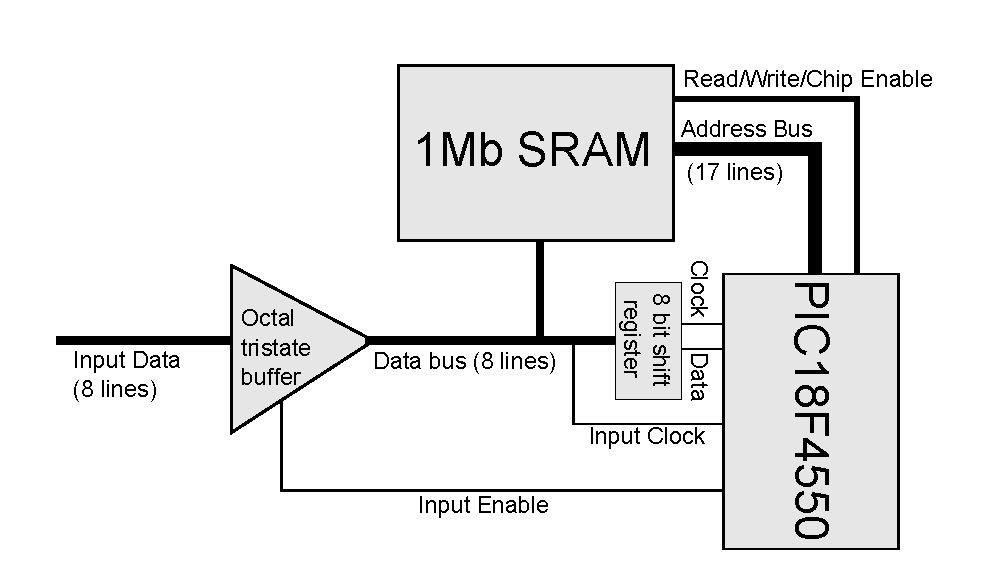
\includegraphics[height=8cm]{hardware.pdf}
    \caption{Capture Hardware}
    \label{fig:app}
    \end{figure}

    \begin{figure}
    \centering
    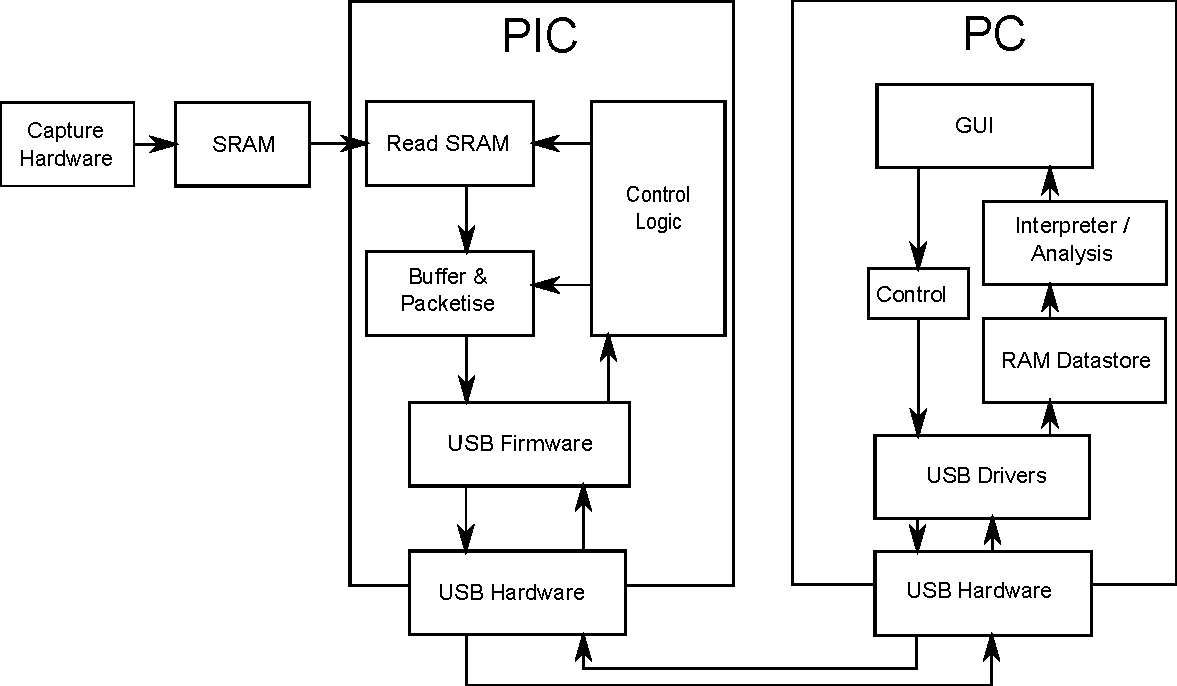
\includegraphics[height=8cm]{block-diagram.pdf}
    \caption{System Block Diagram}
    \label{fig:app}
    \end{figure}

\section{Project Management}
\subsection{Source Control}
    We will be using the ``git'' version control system for source management for both the firmware and software, and Github Issues for issue tracking.

    Jon will be working on the MCU firmware design and implementation and David on the computer software and user interface. Work will be shared on the hardware design and construction.
	
% Now print the appendix section
\appendix
\appendixpage
\addappheadtotoc

\section{Bill of Materials}
    All parts are from Farnell Onecall and prices are list, pre-discount.

    \begin{table}
    \begin{center}
    \begin{tabular}{|r|c|c|c|}
        \hline \textbf{Part No.} & \textbf{Description} & \textbf{Qty} & \textbf{Price/£ }  \\
        \hline 380365 & 74HC165 PISO Shift Register & 1 & 0.38 \\
        \hline 1562896 & Alliance 1Mbit SRAM & 1 & 2.44 \\
         \hline 382449 & 74HCT573 Octal Latch & 1 & 0.58 \\
        \hline 1750143 & Quad Operational Amplifier & 2 & 0.15 \\
        \hline 1841236 & SIL 0.1" 32-way header & 1 & 1.88 \\
        \hline 1667501 & SIL 0.1" 32-way socket & 1 & 3.82 \\
        \hline
    \end{tabular}
    \end{center}
    \caption{Bill of materials for the logic analyser (Appendix A)}
    \label{fig:myt}
    \end{table}

\section{Schematic}
\label{app-schematic}
			
    \begin{figure}
    \centering
    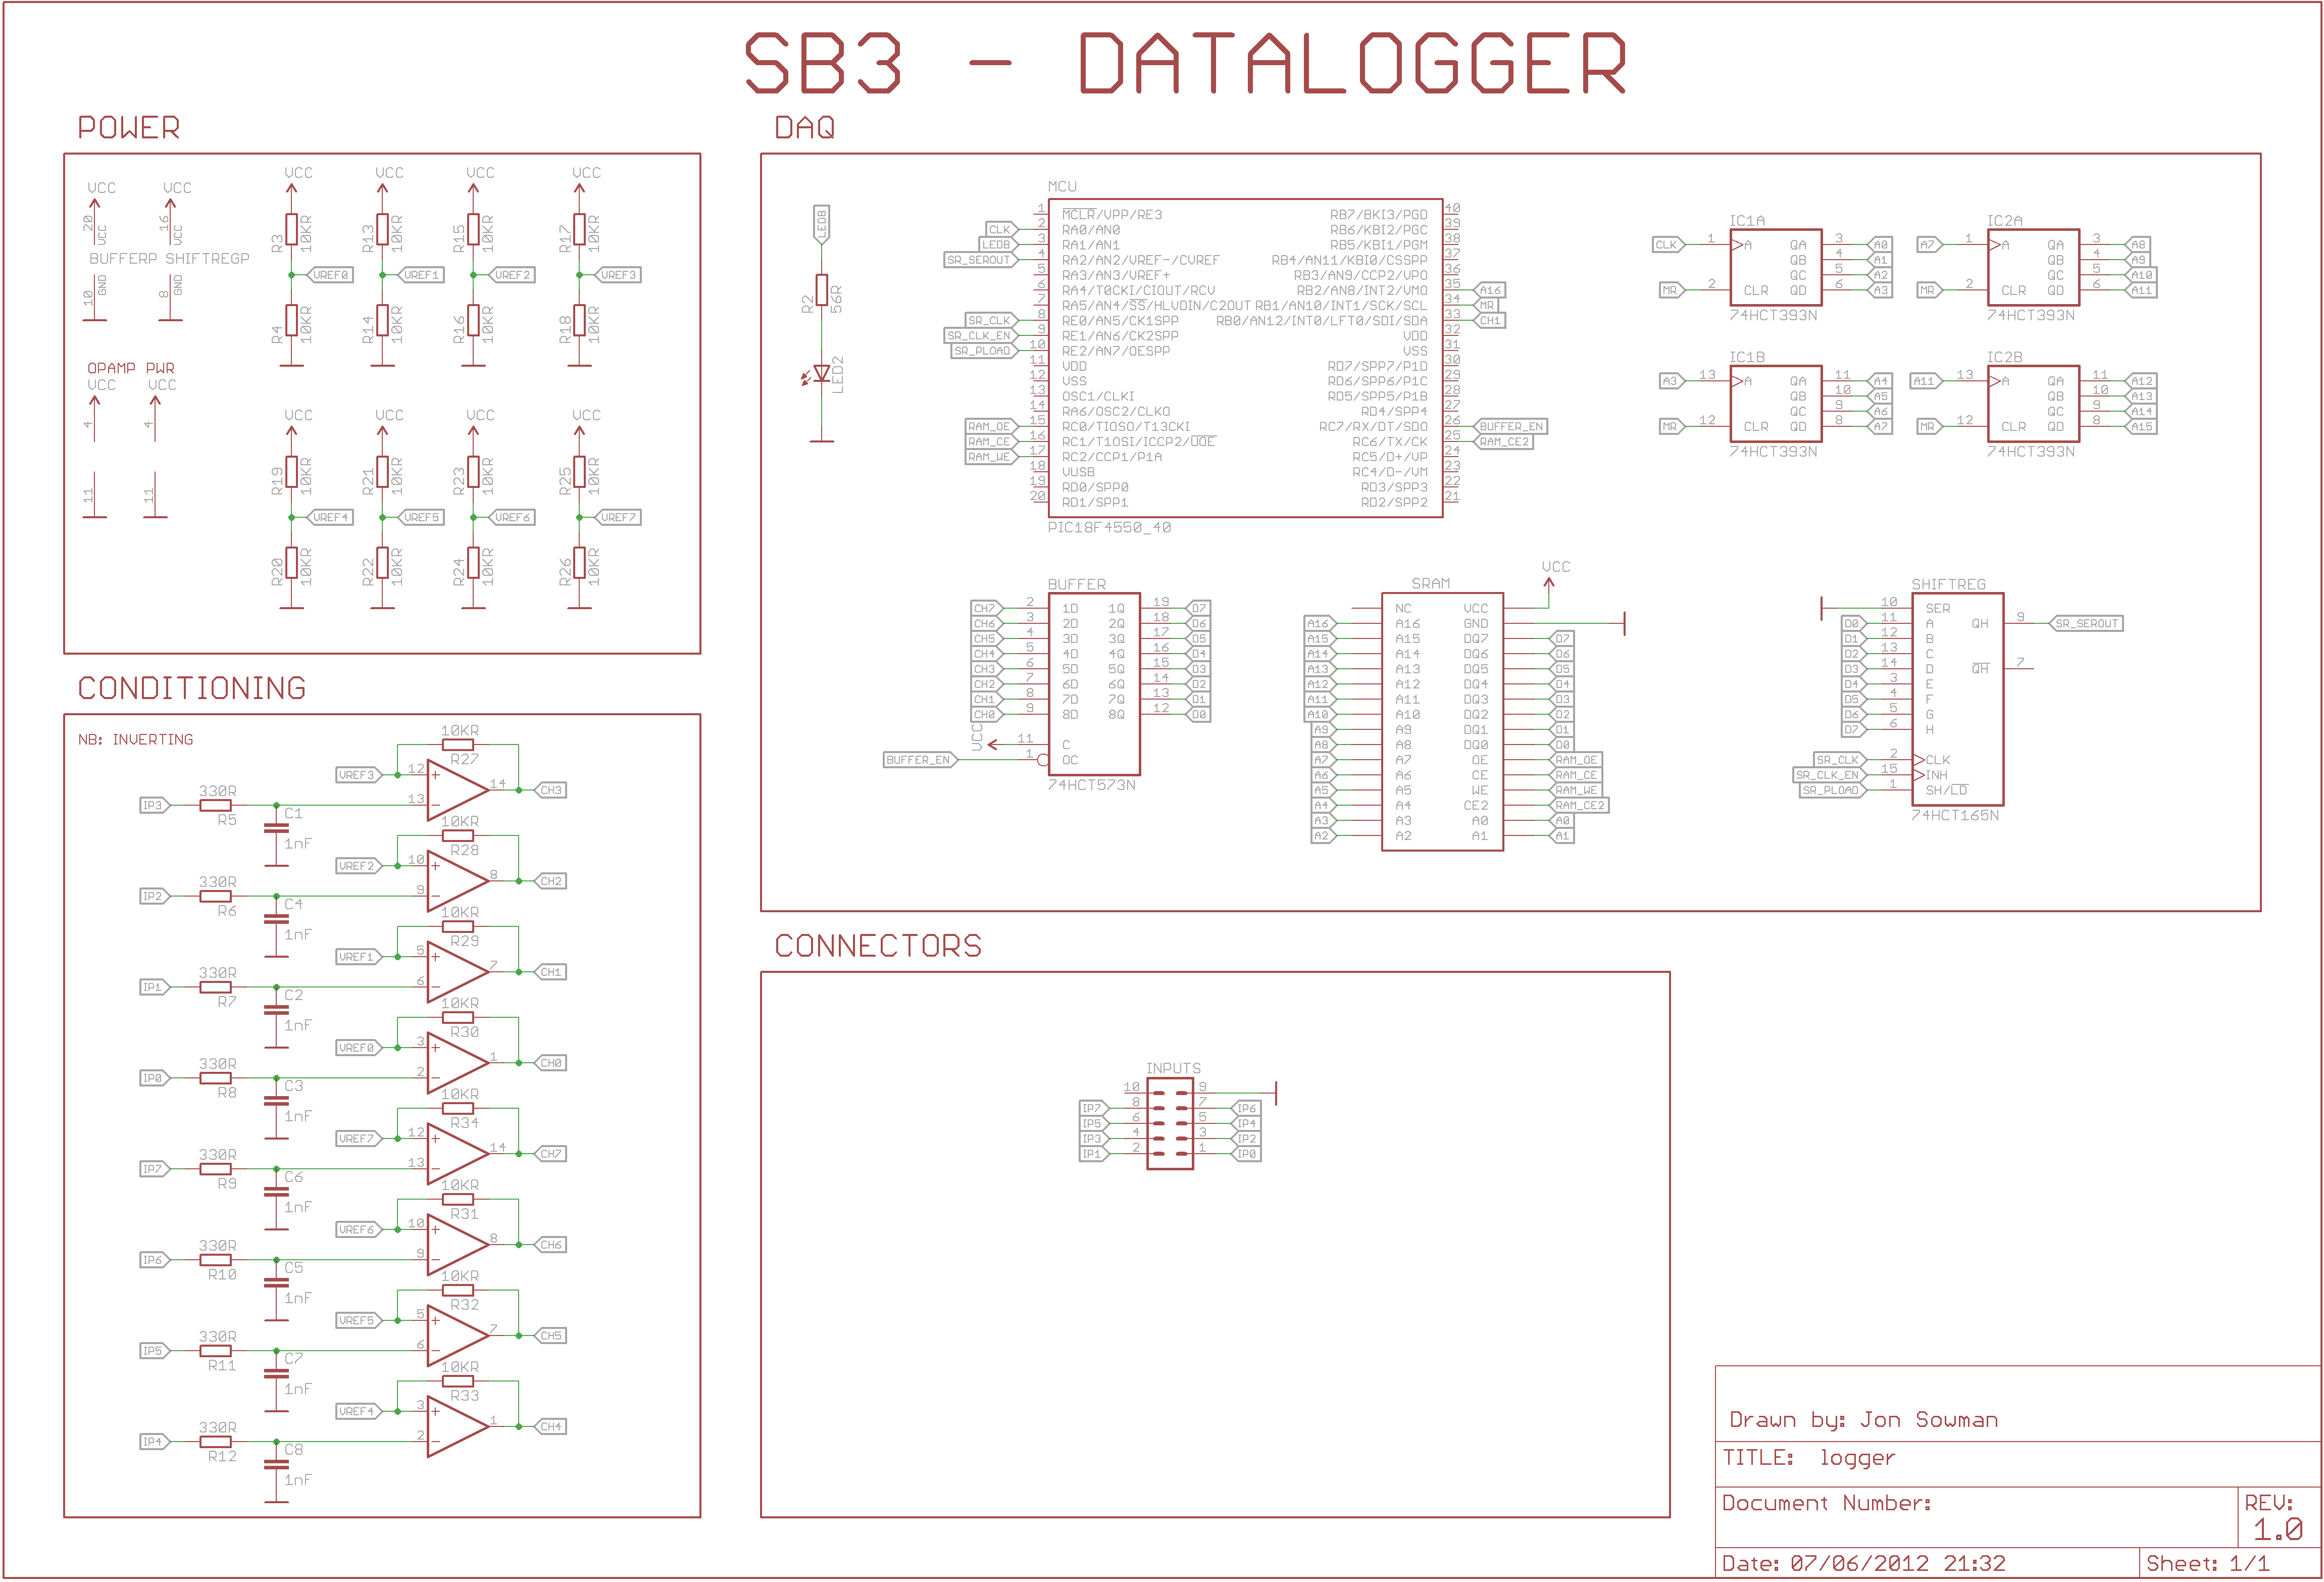
\includegraphics[height=17cm,angle=90]{../../hardware/schematic.png}
    \caption{Logic analyser schematic (Appendix B)}
    \label{fig:sch}
    \end{figure}


\end{document}
